%%%%%%%%%%%%%%%%%%%%%%%%%%%%%%%%%%%%%%%%%
% Beamer Presentation
% LaTeX Template
% Version 1.0 (10/11/12)
%
% This template has been downloaded from:
% http://www.LaTeXTemplates.com
%
% License:
% CC BY-NC-SA 3.0 (http://creativecommons.org/licenses/by-nc-sa/3.0/)
%
%%%%%%%%%%%%%%%%%%%%%%%%%%%%%%%%%%%%%%%%%

%----------------------------------------------------------------------------------------
%	PACKAGES AND THEMES
%----------------------------------------------------------------------------------------

\documentclass{beamer}

\mode<presentation> {

% The Beamer class comes with a number of default slide themes
% which change the colors and layouts of slides. Below this is a list
% of all the themes, uncomment each in turn to see what they look like.

%\usetheme{default}
%\usetheme{AnnArbor}
%\usetheme{Antibes}
%\usetheme{Bergen}
%\usetheme{Berkeley}
%\usetheme{Berlin}
%\usetheme{Boadilla}
%\usetheme{CambridgeUS}
%\usetheme{Copenhagen}
%\usetheme{Darmstadt}
%\usetheme{Dresden}
%\usetheme{Frankfurt}
%\usetheme{Goettingen}
%\usetheme{Hannover}
%\usetheme{Ilmenau}
%\usetheme{JuanLesPins}
%\usetheme{Luebeck}
\usetheme{Madrid}
%\usetheme{Malmoe}
%\usetheme{Marburg}
%\usetheme{Montpellier}
%\usetheme{PaloAlto}
%\usetheme{Pittsburgh}
%\usetheme{Rochester}
%\usetheme{Singapore}
%\usetheme{Szeged}
%\usetheme{Warsaw}

% As well as themes, the Beamer class has a number of color themes
% for any slide theme. Uncomment each of these in turn to see how it
% changes the colors of your current slide theme.

%\usecolortheme{albatross}
%\usecolortheme{beaver}
%\usecolortheme{beetle}
%\usecolortheme{crane}
%\usecolortheme{dolphin}
%\usecolortheme{dove}
%\usecolortheme{fly}
%\usecolortheme{lily}
%\usecolortheme{orchid}
%\usecolortheme{rose}
%\usecolortheme{seagull}
%\usecolortheme{seahorse}
%\usecolortheme{whale}
%\usecolortheme{wolverine}

%\setbeamertemplate{footline} % To remove the footer line in all slides uncomment this line
%\setbeamertemplate{footline}[page number] % To replace the footer line in all slides with a simple slide count uncomment this line

\setbeamertemplate{navigation symbols}{} % To remove the navigation symbols from the bottom of all slides uncomment this line
}

\usepackage{graphicx} % Allows including images
\usepackage{booktabs} % Allows the use of \toprule, \midrule and \bottomrule in tables
\usepackage{selinput}      % Halbautomatische Auswahl der Eingabecodierung
\SelectInputMappings{      % mit Hilfe ausgewählter Glyphen
  adieresis={ä},	   % siehe: http://partners.adobe.com/public/developer/en/opentype/glyphlist.txt
  germandbls={ß},
  Euro={€}
}

%----------------------------------------------------------------------------------------
%	TITLE PAGE
%----------------------------------------------------------------------------------------

\title[E/A-Leistungsvorhersage im HPC]{Vorhersage von E/A-Leistung im Hochleistungsrechnen unter der Verwendung von neuronalen Netzen} % The short title appears at the bottom of every slide, the full title is only on the title page

\author{Jan Fabian Schmid} % Your name
\institute[UHH] % Your institution as it will appear on the bottom of every slide, may be shorthand to save space
{
Universität Hamburg \\ % Your institution for the title page
\medskip
\textit{2schmid@informatik.uni-hamburg.de} % Your email address
}
\date{\today} % Date, can be changed to a custom date

\begin{document}

\begin{frame}
\titlepage % Print the title page as the first slide
\end{frame}

\begin{frame}
\frametitle{Übersicht} % Table of contents slide, comment this block out to remove it
\tableofcontents % Throughout your presentation, if you choose to use \section{} and \subsection{} commands, these will automatically be printed on this slide as an overview of your presentation
\end{frame}

%----------------------------------------------------------------------------------------
%	PRESENTATION SLIDES
%----------------------------------------------------------------------------------------

\section{Motivation}
\begin{frame}
\frametitle{Motivation}
\begin{itemize}
	\item Hocheleistungsrechnen bekommt zunehmende Bedeutung in der Wissenschaft
	%Simulation komplexer abstrakter Modelle in verschiedenen Bereichen 	
	%Mehrkörpersimulationen in der Astronomie, für Strömungssimulationen oder zur Berechnung von Klimaprognosen
	\pause
	\item Verwendung massiv paralleler Systeme
	%Flaschenhals einzelner Hardwarekomponenten umgehen
	%Aufwendige Programmierung
	\pause	
	\item Unterstützung der Wissenschaftler durch Werkzeuge
	%Fehlerdiagnostik, Leistungsanalyse, Visualisierung des Programms und der Ergebnisse, sowie zum Parallelisieren des Programmcodes
	%möglichst autonome Optimierungen, Wissenschaftler kann sich aufs wesentliche konzentrieren
	\pause
	\item Analysewerkzeug zur Beurteilung der Effizienz der Ein-/Ausgabe (E/A) eines Programms
	%insbesondere die Vermeidung von Festplattenzugriffen
	\begin{itemize}
		\pause
		\item Modellerstellung
		%Modell erstellen, um E/A-System besser verstehen zu können
		\pause		
		\item Kategorisierung von E/A-Leistung
		%Anteil an Festplattenzugriffen etc. abschätzen, dadurch Beurteilung der Effizienz möglich
	\end{itemize}			
\end{itemize}
\end{frame}

\section{Verwandte Arbeiten}
%black vs white-box
\begin{frame}
\frametitle{Verwandte Arbeiten}
\begin{itemize}
	\item Betrachtung von Systemen mit einzelnen Festplatten
	%keine Verbünde, sondern nur die E/A-Leistung einzelner Platten wird vorhergesagt
	\item White-Box-Modellierung
	\begin{itemize}
		\item Modellbildung mit Kenntnis von Hardwaredetails
		\item Nachbildung der internen Verarbeitung
		%Latenzzeiten, Rotationsgeschw. von Platte, Geschw. des Lesekopfes
		\item Sehr aufwendig zu konfigurieren
		%praktisch nur für einzelne Festplatten möglich
		\item Sehr präzise Vorhesagen
		%Wenn korrekt und detailiert modelliert wurde	
	\end{itemize}
	\item Black-Box-Modellierung
	\begin{itemize}
		\item Modellbildung ohne Kenntnis von Hardwaredetails
		%Nur Messwerte können verwendet werden
		\item mathematische Beschreibung mittels Regressionsanalyse
		%kein Nachbildung oder Wissen von internen Vorgängen
		%verschiedene statistische Methoden (maschinelles Lernen) können verwendet werden
		\item Einfach und flexibel einsetzbar
		%Ein Modell für viele Systeme verwendbar
		\item Nicht so präzise Vorhersagen
	\end{itemize}
\end{itemize}
\end{frame}

\section{Künstliche neuronale Netze}
\begin{frame}
\frametitle{Künstliche neuronale Netze}
\begin{columns}
\column{.45\textwidth}
\begin{itemize}
	\item Verfahren des maschinellen Lernens
	\begin{itemize}
		\item Überwachtes Lernen
		%Vorgabe von Ausgabewerten als Lösungen
		\item Trainingsdatensatz
		%Beim Lernvorgang verwendete Daten
		\item Testdatensatz
		%ungesehene Daten zur Überprüfung der Abstraktionsfähigkeit des Modells
	\end{itemize}
	\item Zur Regressionsanalyse verwendet
	%Bestimmung der Zusammenhänge der Attribute des Eingabevektors zu den Attributen des Ausgabevektors
	%Bild einfaches feedforward-Netz, eingabevektor mit 2 attributen, ausgabevektor mit einem, und 2 verdeckten schichten
	\item Trainieren durch Fehlerrückführung (engl. backpropagation)
	%mittlere quadratische Fehler gegenüber idealer Ausgabe berechnen und mit Gradientenverfahren Gewichtsupdate berechnen
\end{itemize}

\column{.45\textwidth}
\begin{figure}
	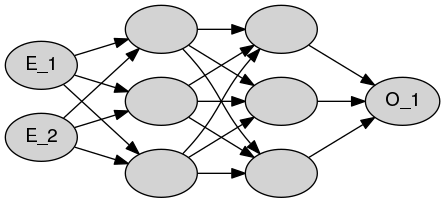
\includegraphics[width=0.9\linewidth]{Bilder/netz.png}
\end{figure}

\begin{figure}
	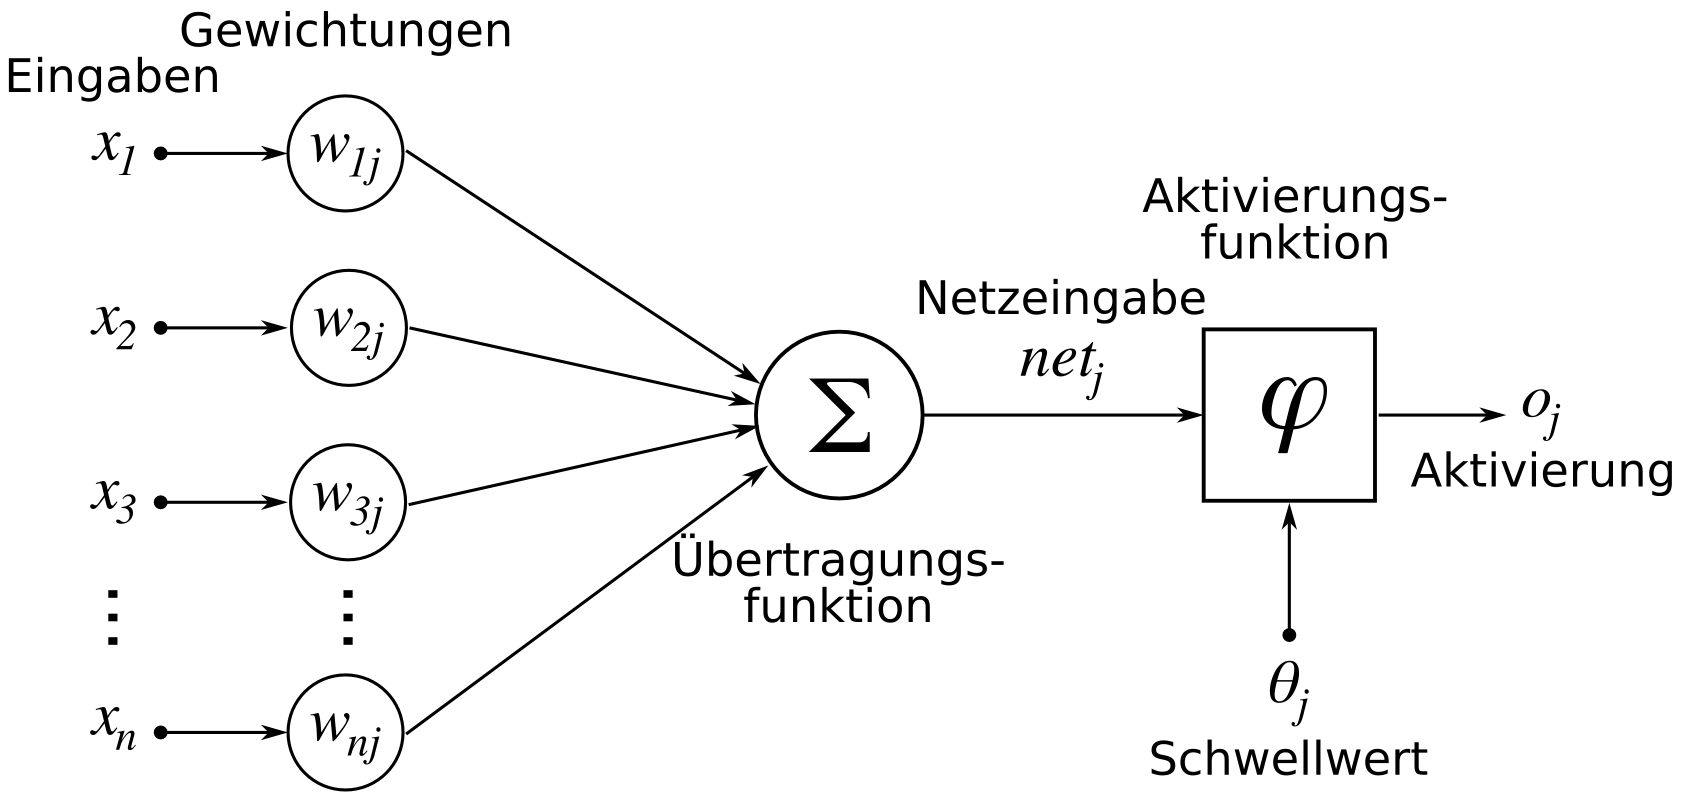
\includegraphics[width=1\linewidth]{Bilder/ArtificialNeuronModel_deutsch.png}
\end{figure}
\end{columns}
\end{frame}

\begin{frame}
\frametitle{Künstliche neuronale Netze}
\begin{columns}
\column{.45\textwidth}
\begin{itemize}
	\item Mächtiger als lineare Regression
	%Mit ausreichender Komplexität des Netzes Approximation beliebiger kontinuierlicher Funktionen
	%universal approximation theorem von Cybenko
\end{itemize}

\column{.45\textwidth}
\begin{figure}
	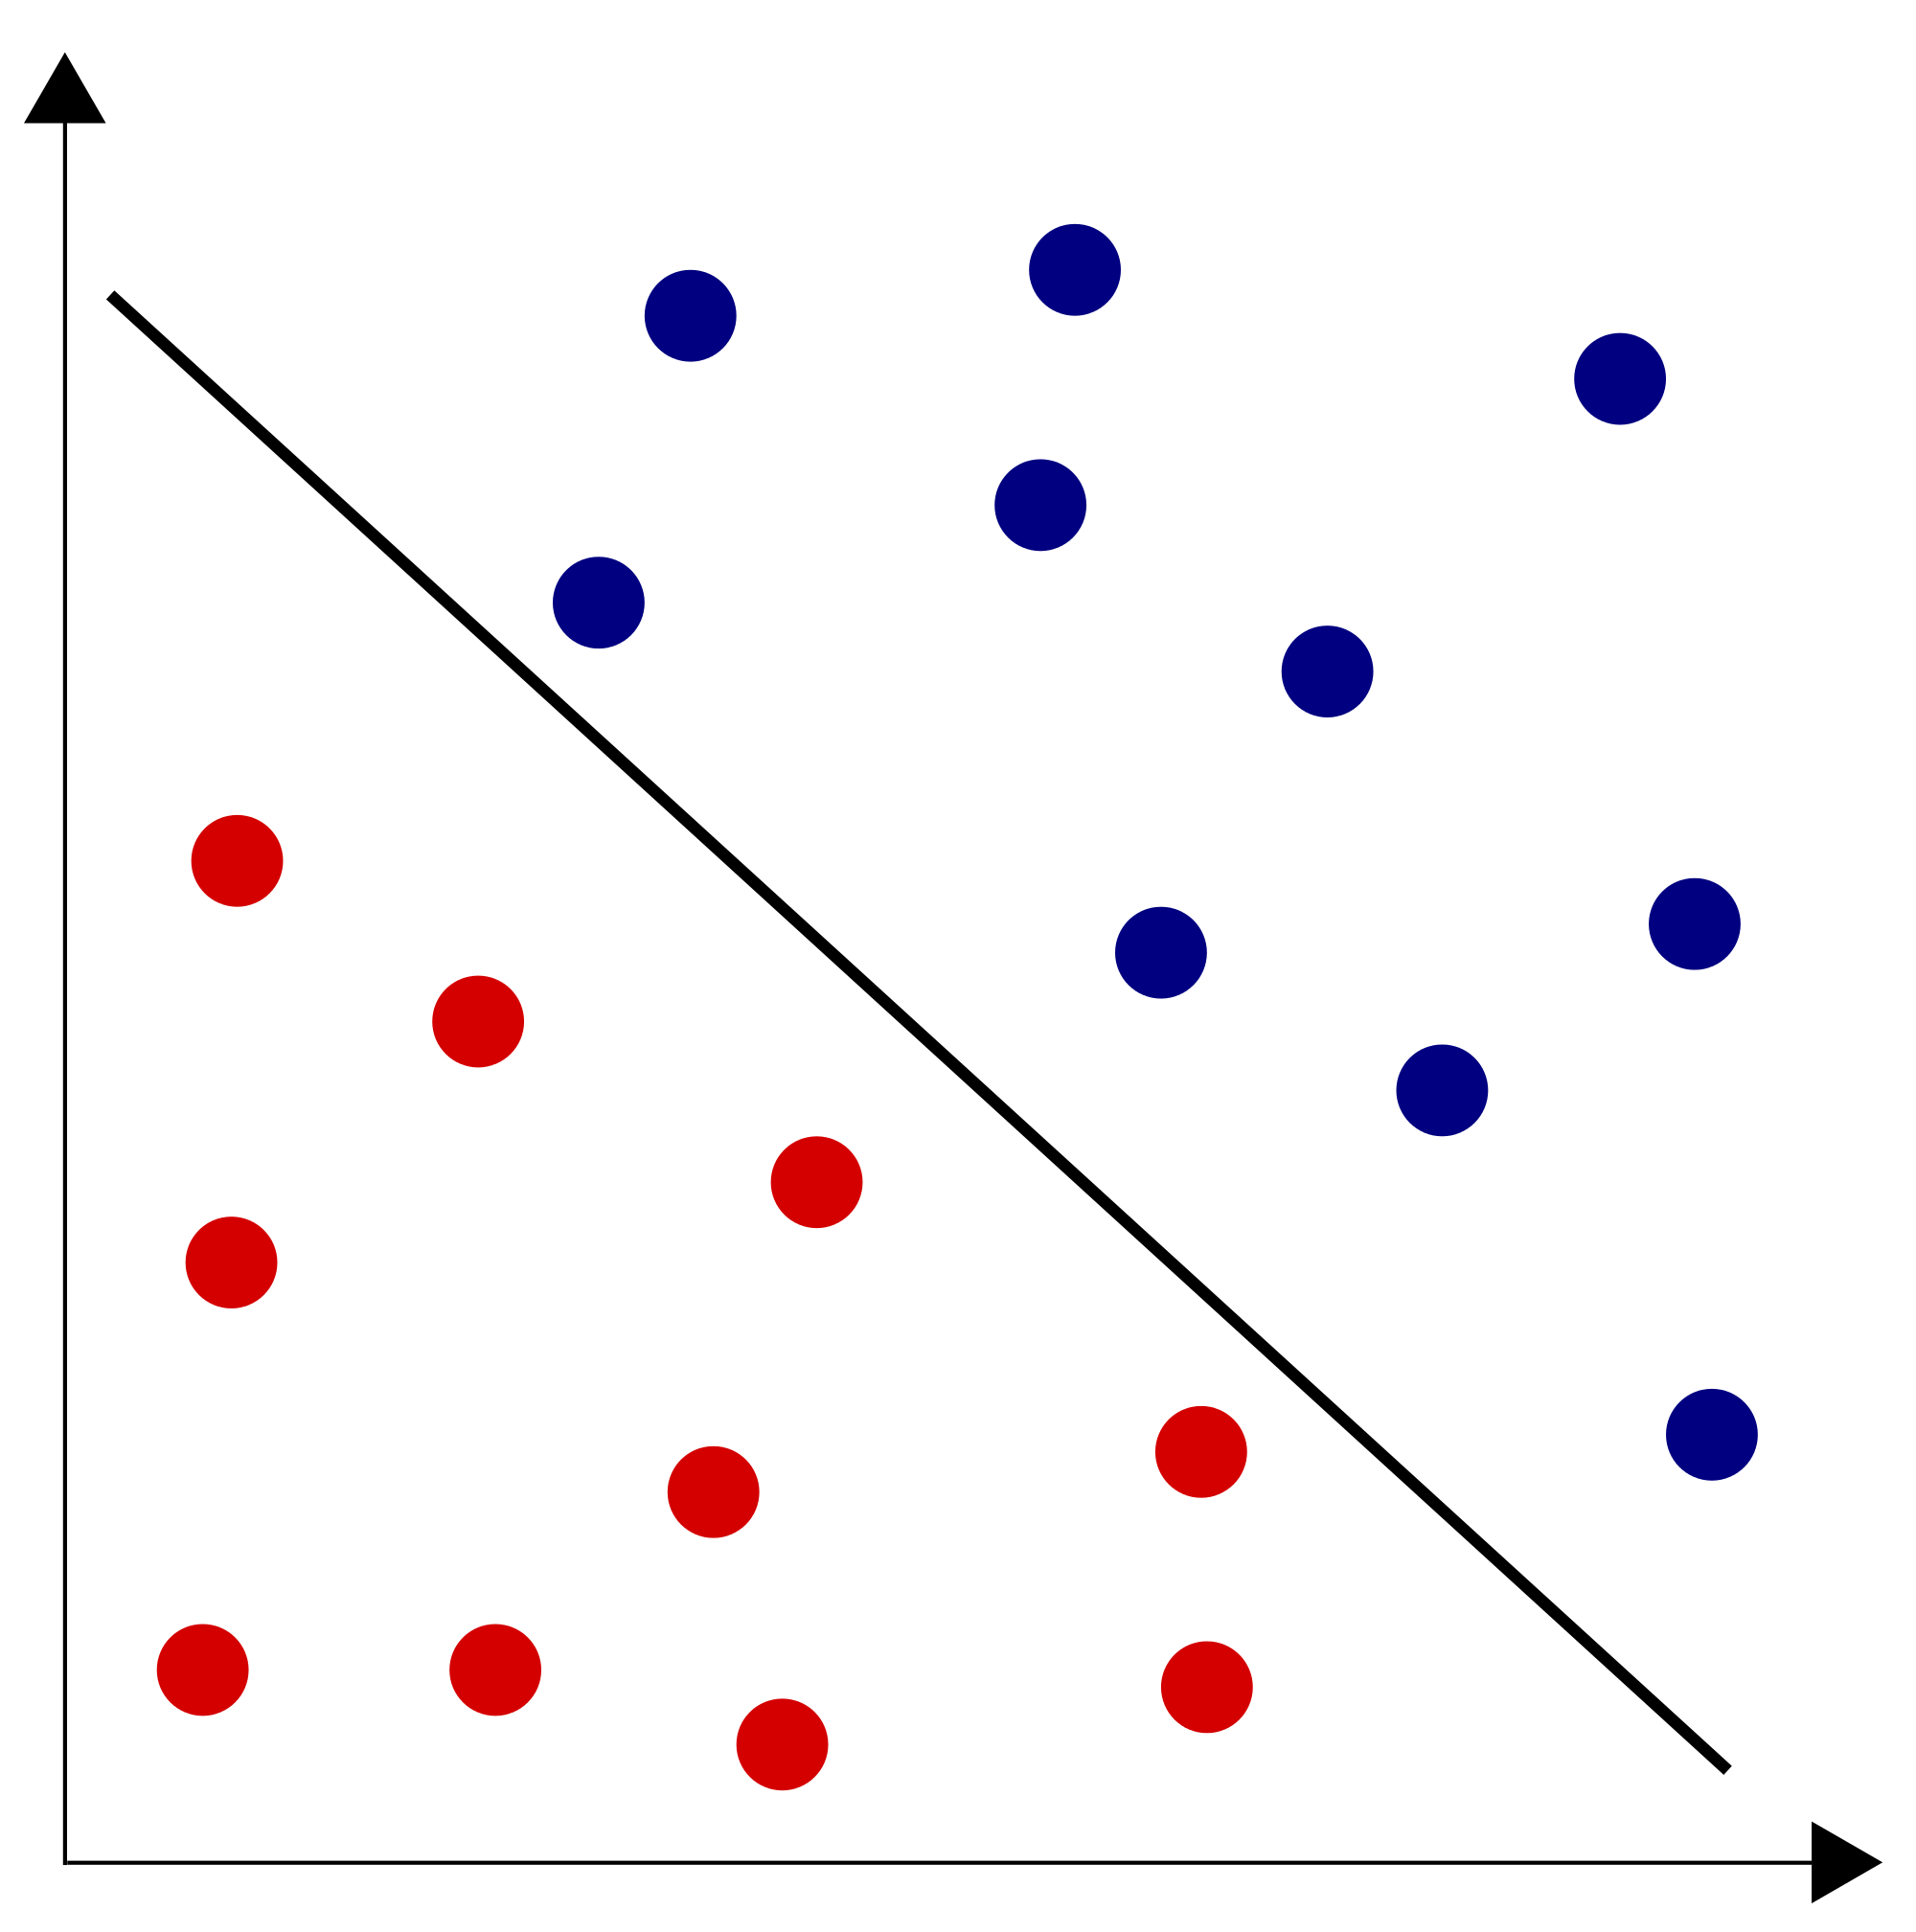
\includegraphics[width=0.45\linewidth]{Bilder/2000px-Separability_YES.png}
\end{figure}
\begin{figure}
	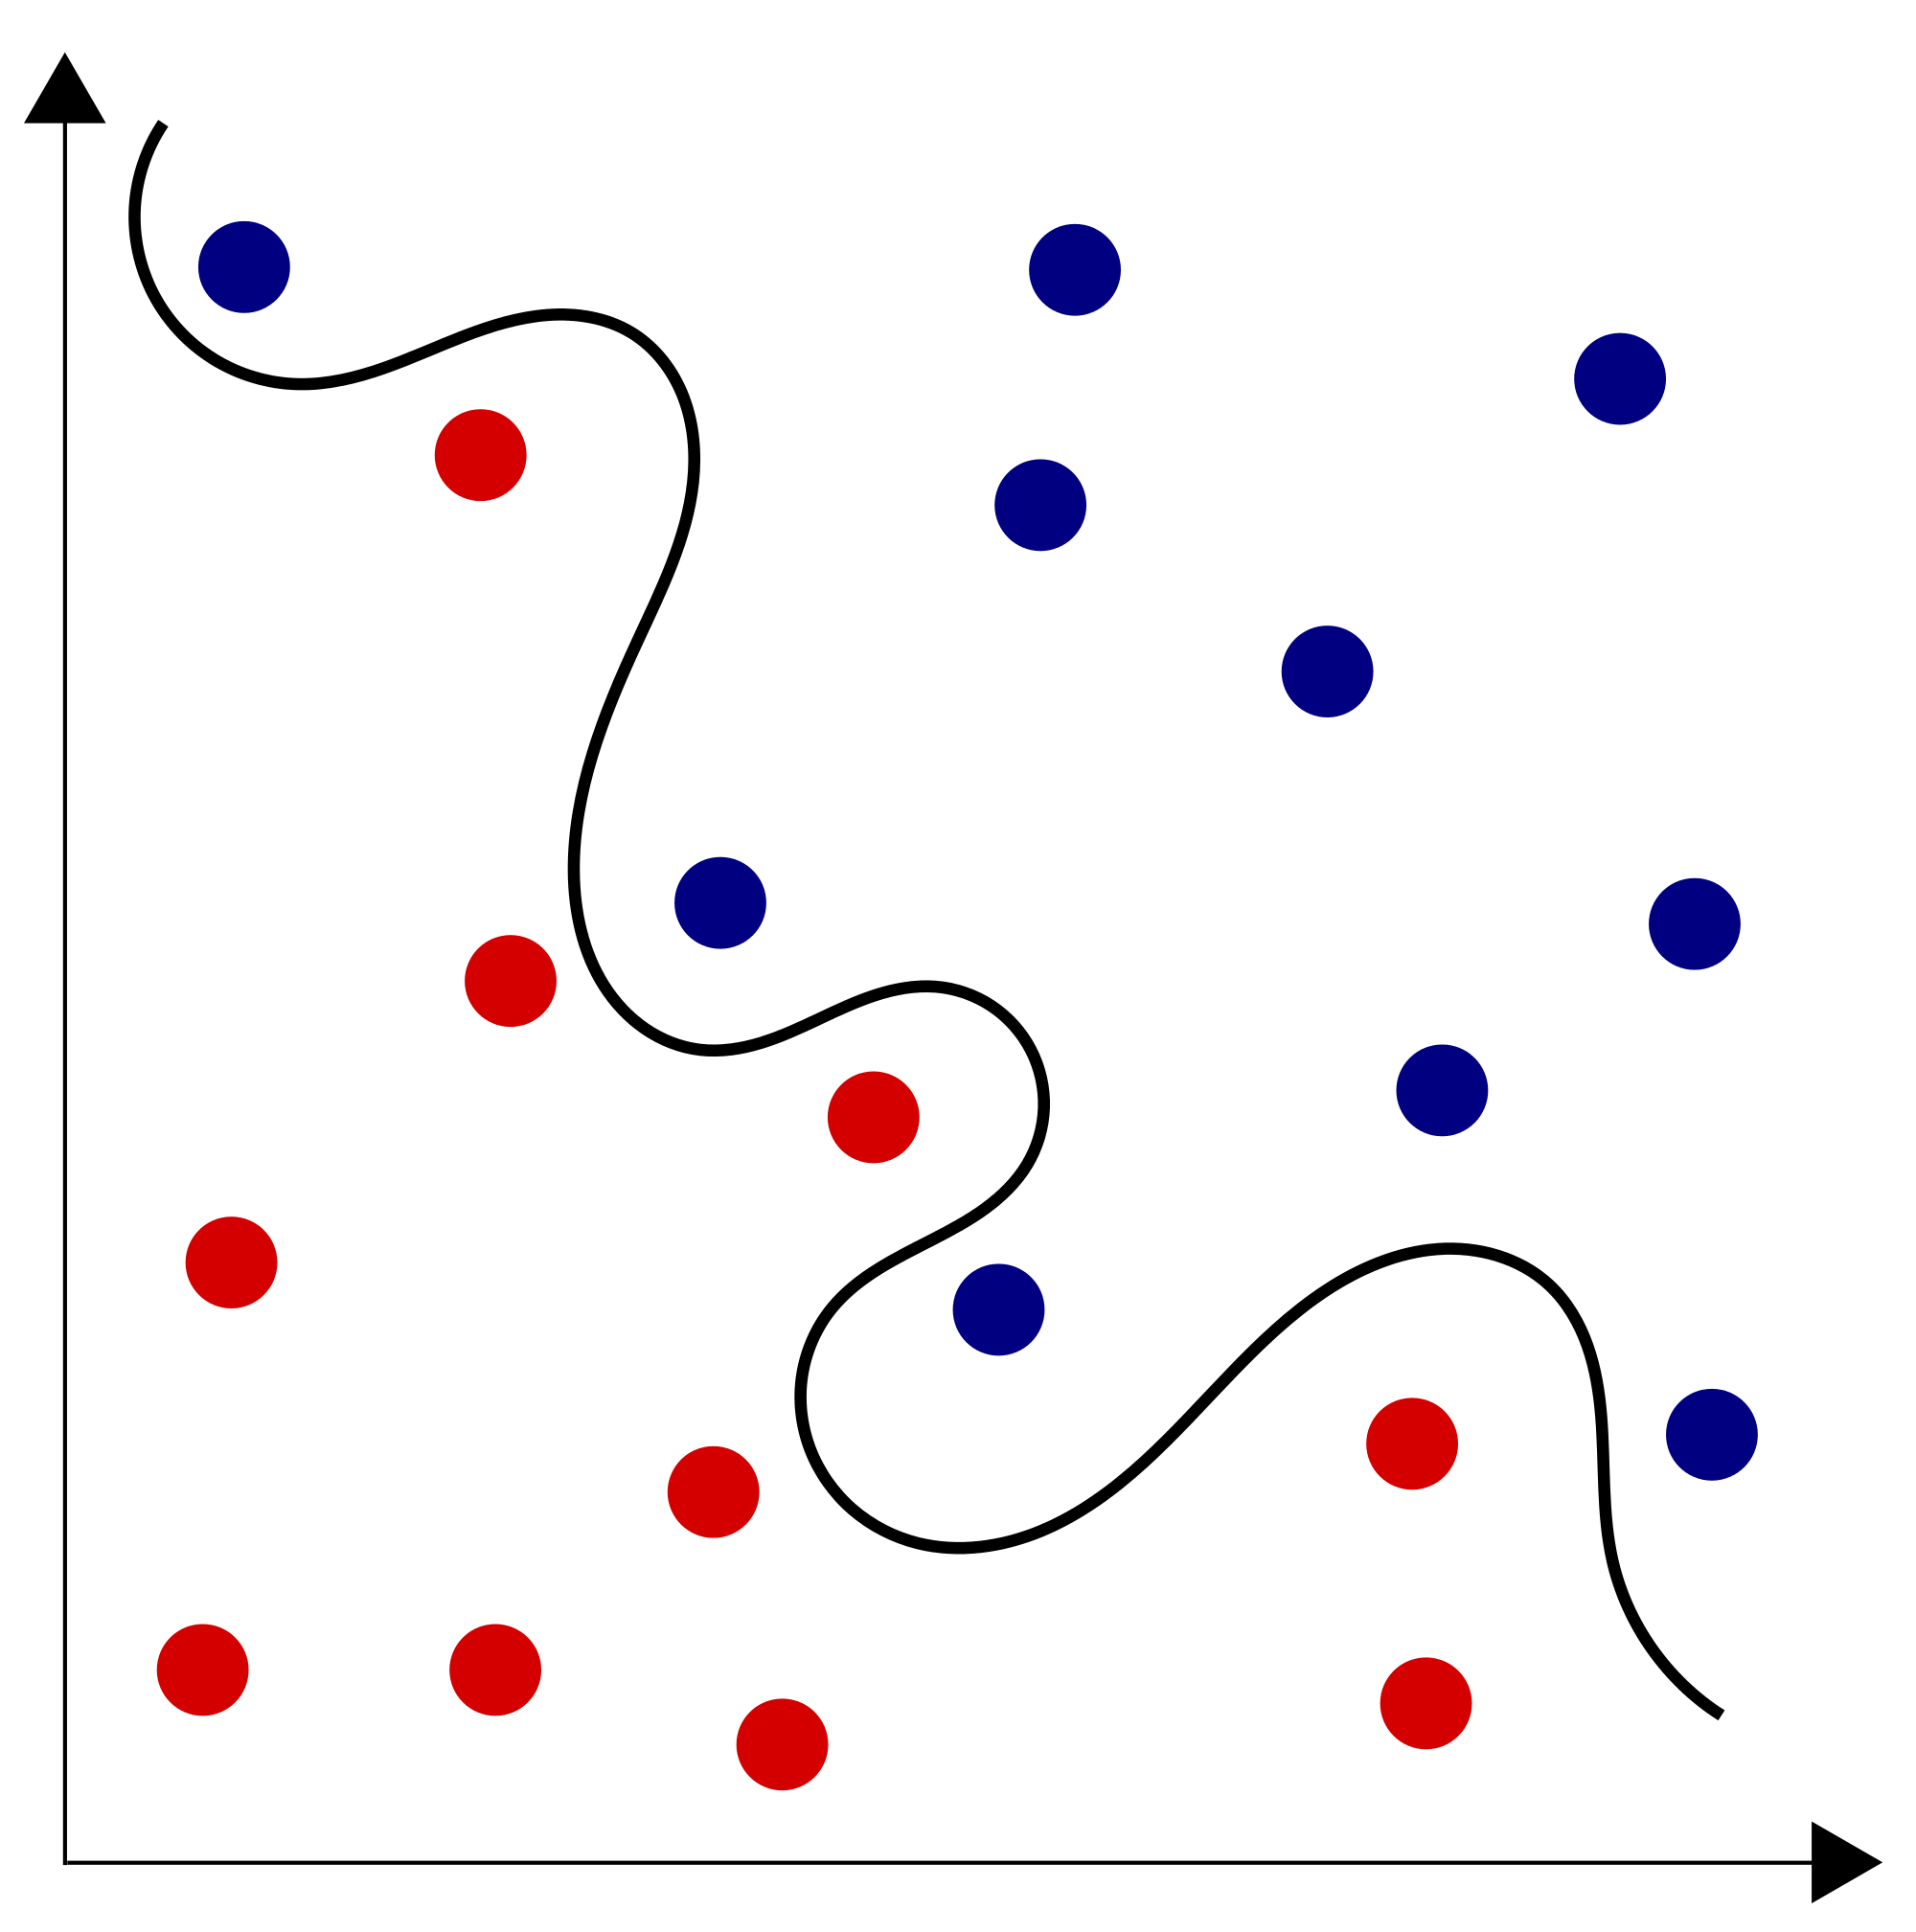
\includegraphics[width=0.45\linewidth]{Bilder/2000px-Separability_NO.png}
\end{figure}
\end{columns}
\end{frame}

\section{Gestaltung der Analyse}
\subsection{Modell des Ein-/Ausgabe-Pfads}
%speicherhierachie, Zugriffszeit davon abhängig
\begin{frame}
\frametitle{Gestaltung der Analyse: Modell des Ein-/Ausgabe-Pfads}
\begin{columns}
\column{.45\textwidth}
\begin{itemize}
	\item<1-> Speicherhierachie
	%System entspricht einer Hierachie von verschiedenen Speichermedien
	\item<2-> Modell des E/A-Systems
	%Unterscheidung von drei Anteilen des Zeitaufwandes zum Bearbeiten einer Anfrage: Festplatten, Netzwerk, Arbeitsspeicher+Caches
	\item<3-> Verarbeitung entlang des E/A-Pfades
	%Pfad abhängig davon wo Daten sich befinden
	%Zeitanteil in den drei Bereichen hängt vom Durchsatz und Latenzen ab
	\item<4-> Zugriffszeit wesentlich durch tiefe des Pfades bestimmt
	%durch Speicherhirachie hängt Verarbeitungszeit von der langsamsten Komponente ab
\end{itemize}

\column{.45\textwidth}
\begin{figure}
	\includegraphics<1->[width=0.8\linewidth]{Bilder/hierachie.png}
\end{figure}
\begin{figure}
	\includegraphics<2>[width=0.8\linewidth]{Bilder/rechnerknoten.png}
	\includegraphics<3>[width=0.8\linewidth]{Bilder/rechnerknoten_ea_pfad.png}
\end{figure}
\end{columns}
\end{frame}

\subsection{Benchmark-Tests}
%welche Messreihen wurden gemacht, auf welchem Rechner, welche Daten stehen zur Verfügung, wie sehen daten aus?
\begin{frame}
\frametitle{Gestaltung der Analyse: Benchmark-Tests}
%System wird mit Messungen untersucht, beschränktes Wissen dabei:
	\begin{itemize}
		\item Messbare/bekannte Attribute des Systems:
		\begin{itemize}
			\item Datei ID
			%zur Identifikation der aufgerufenen Datei
			\item Zugriffsgröße
			%Anazahl Bytes die gelesen/geschrieben werden sollen
			\item Offset
			%Abstand vom Dateibeginn bis zum zugegriffenen Bereich
			\item Delta-Offset = $\text{Offset}[i]-(\text{Offset}[i-1]+\text{Zugriffsgröße}[i-1])$
			%Strecke die Dateizeiger zurücklegen muss			
			\item Operationstyp 
			%lesend oder schreibend
		\end{itemize}
		\item Keine Informationen über internen Zustand des Systems
		%gecached oder nech?
	\end{itemize}
\end{frame}

\begin{frame}
\frametitle{Gestaltung der Analyse: Benchmark-Tests}
%Messreihen und Testsystem
\begin{itemize}
	\item Messreihen und Testsystem
	\item Zwei untersuchte Anwendungsfälle:
	\begin{itemize}
		\item \textbf{SEQ:} Sequentieller Zugriff auf hintereinanderliegende Daten
		\item \textbf{RND:} Zufälliger Zugriffsort 
	\end{itemize}
	\item Jeweils lesende und schreibende Messreihen
	%3 Messreihen pro Anwendungsfall und Zugriffsart
	\item Testsystem: Mistral
	\begin{itemize}
		\item Über 1500 Knoten
		\item Speichersystem Lustre
		\item 30 Petabyte Speicherkapazität
	\end{itemize}
\end{itemize}
\end{frame}

\subsection{Exploration der Messdaten}
\begin{frame}
\frametitle{Gestaltung der Analyse: Exploration der Messdaten}
\begin{columns}
\column{.45\textwidth}
	\begin{figure}
		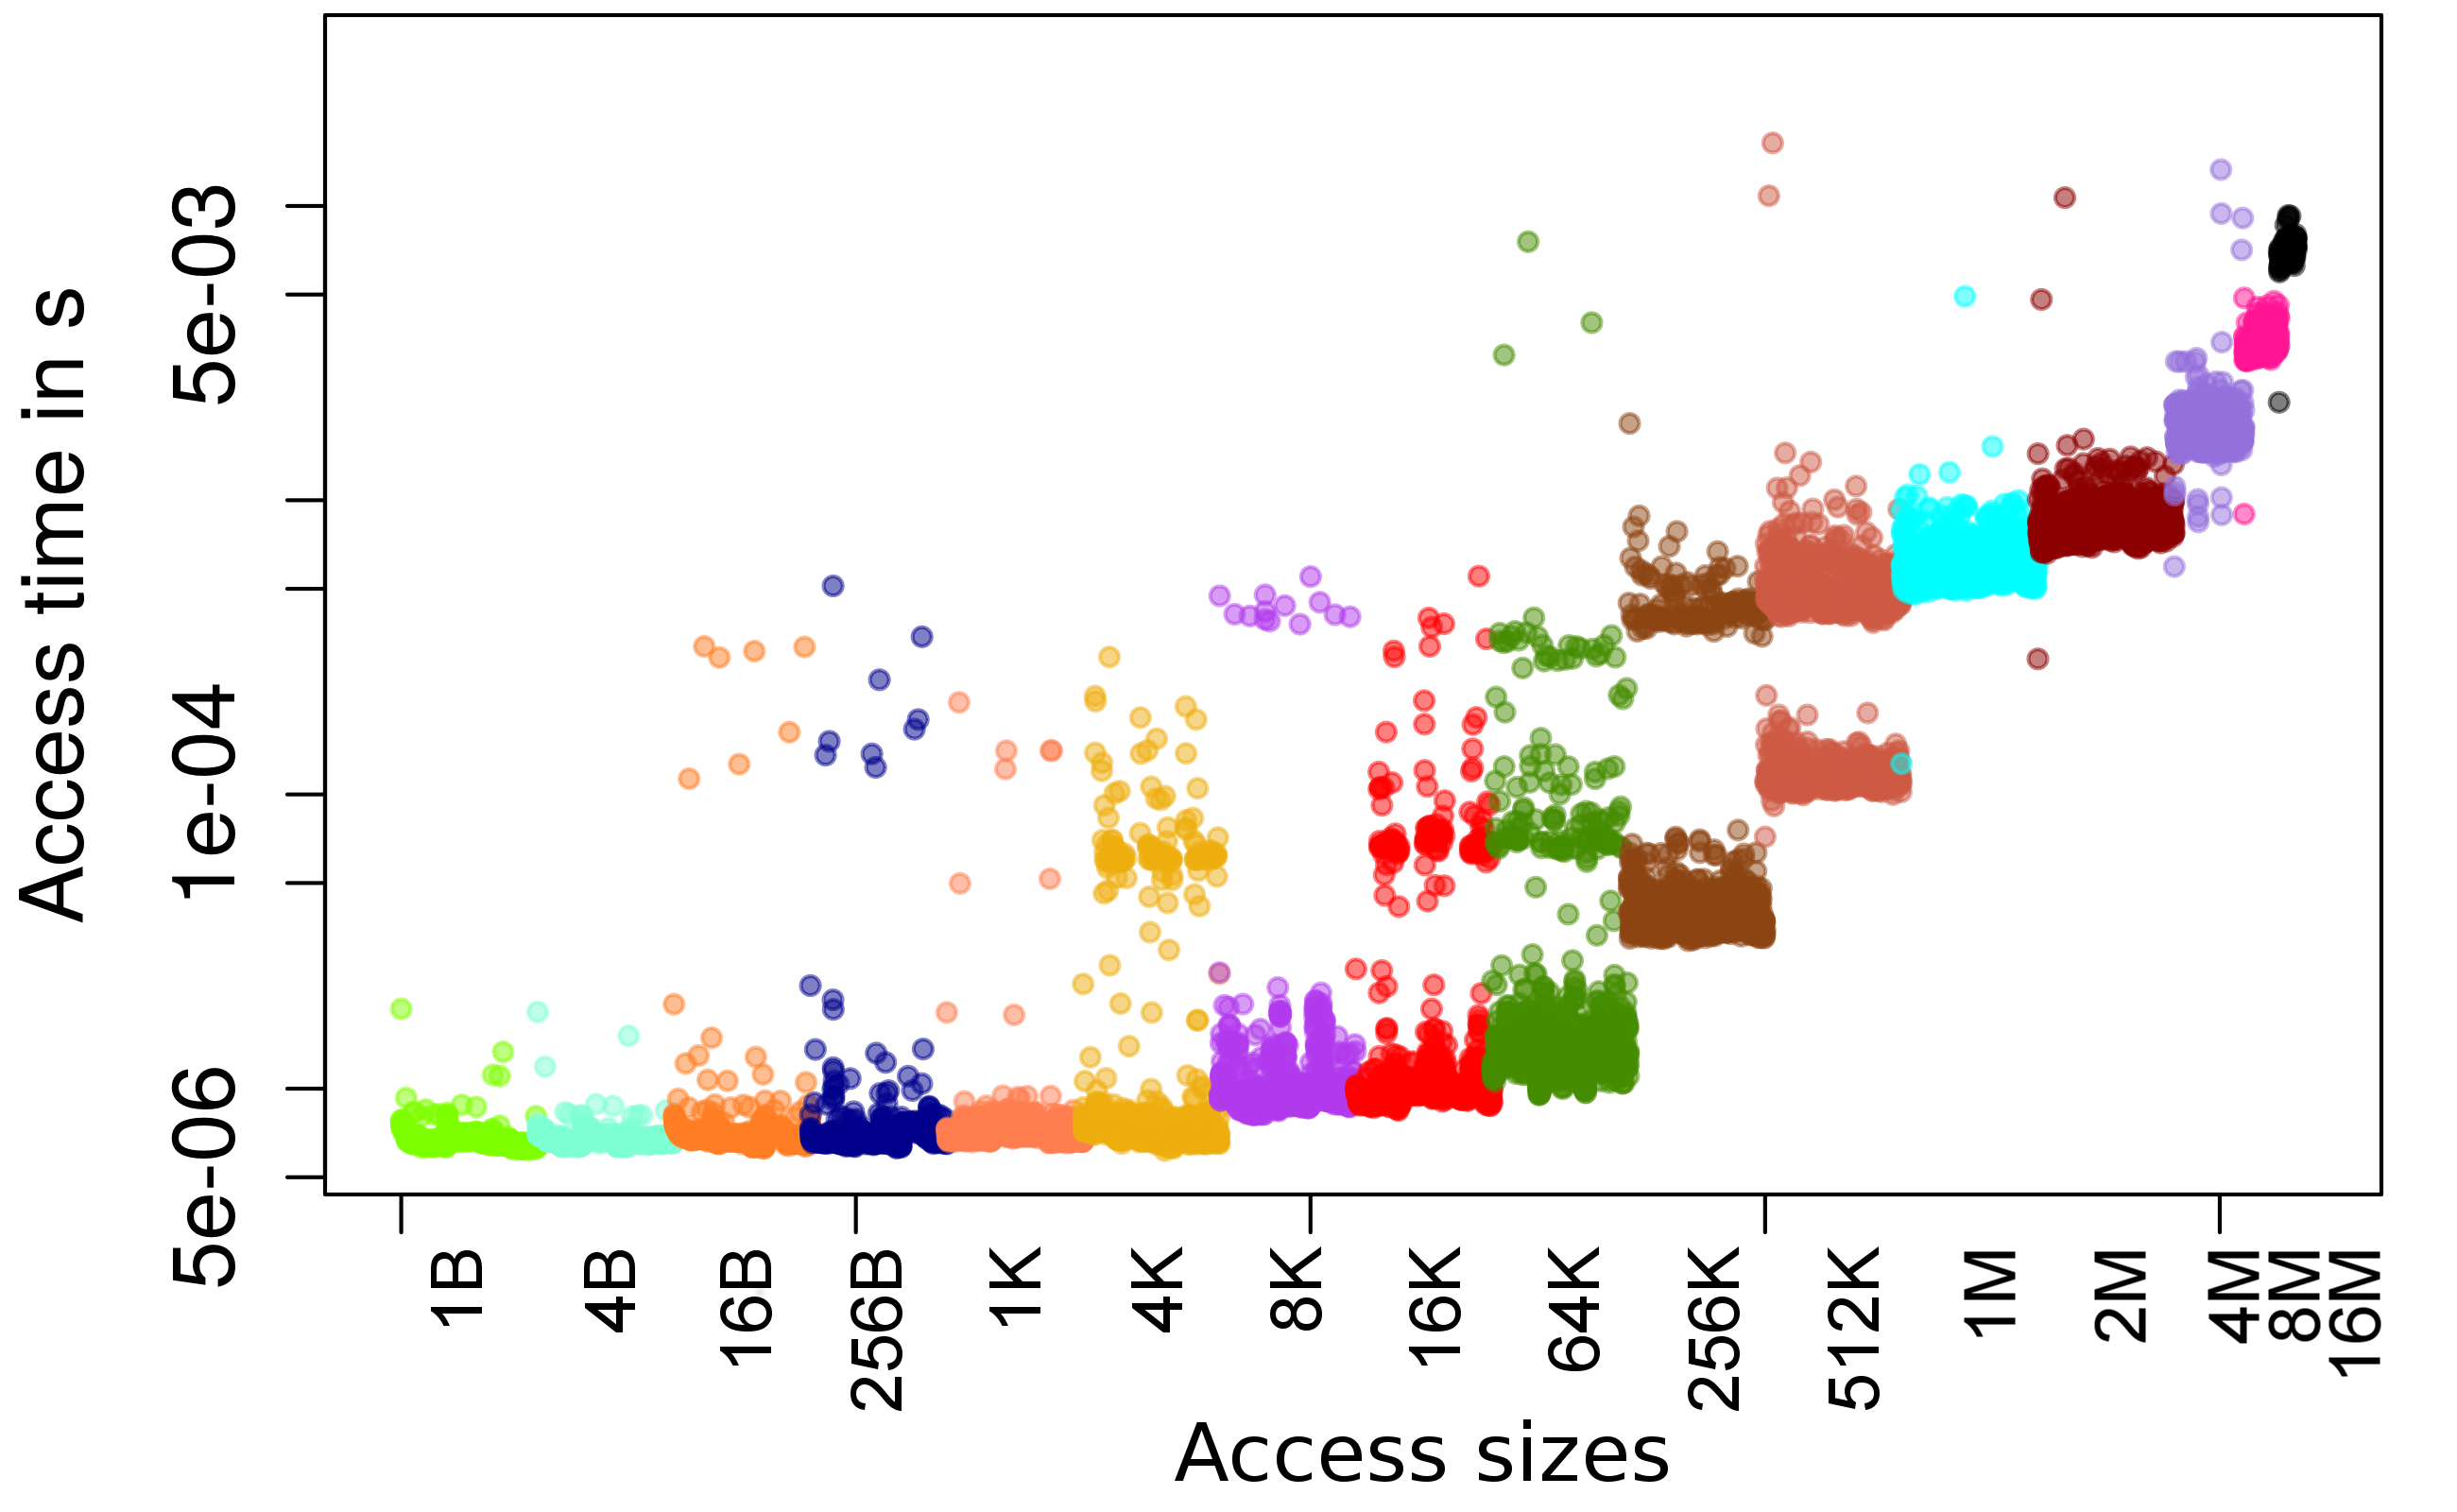
\includegraphics[width=1\linewidth]{Bilder/plot_SizeSorted_log_read_seq.png}\\
		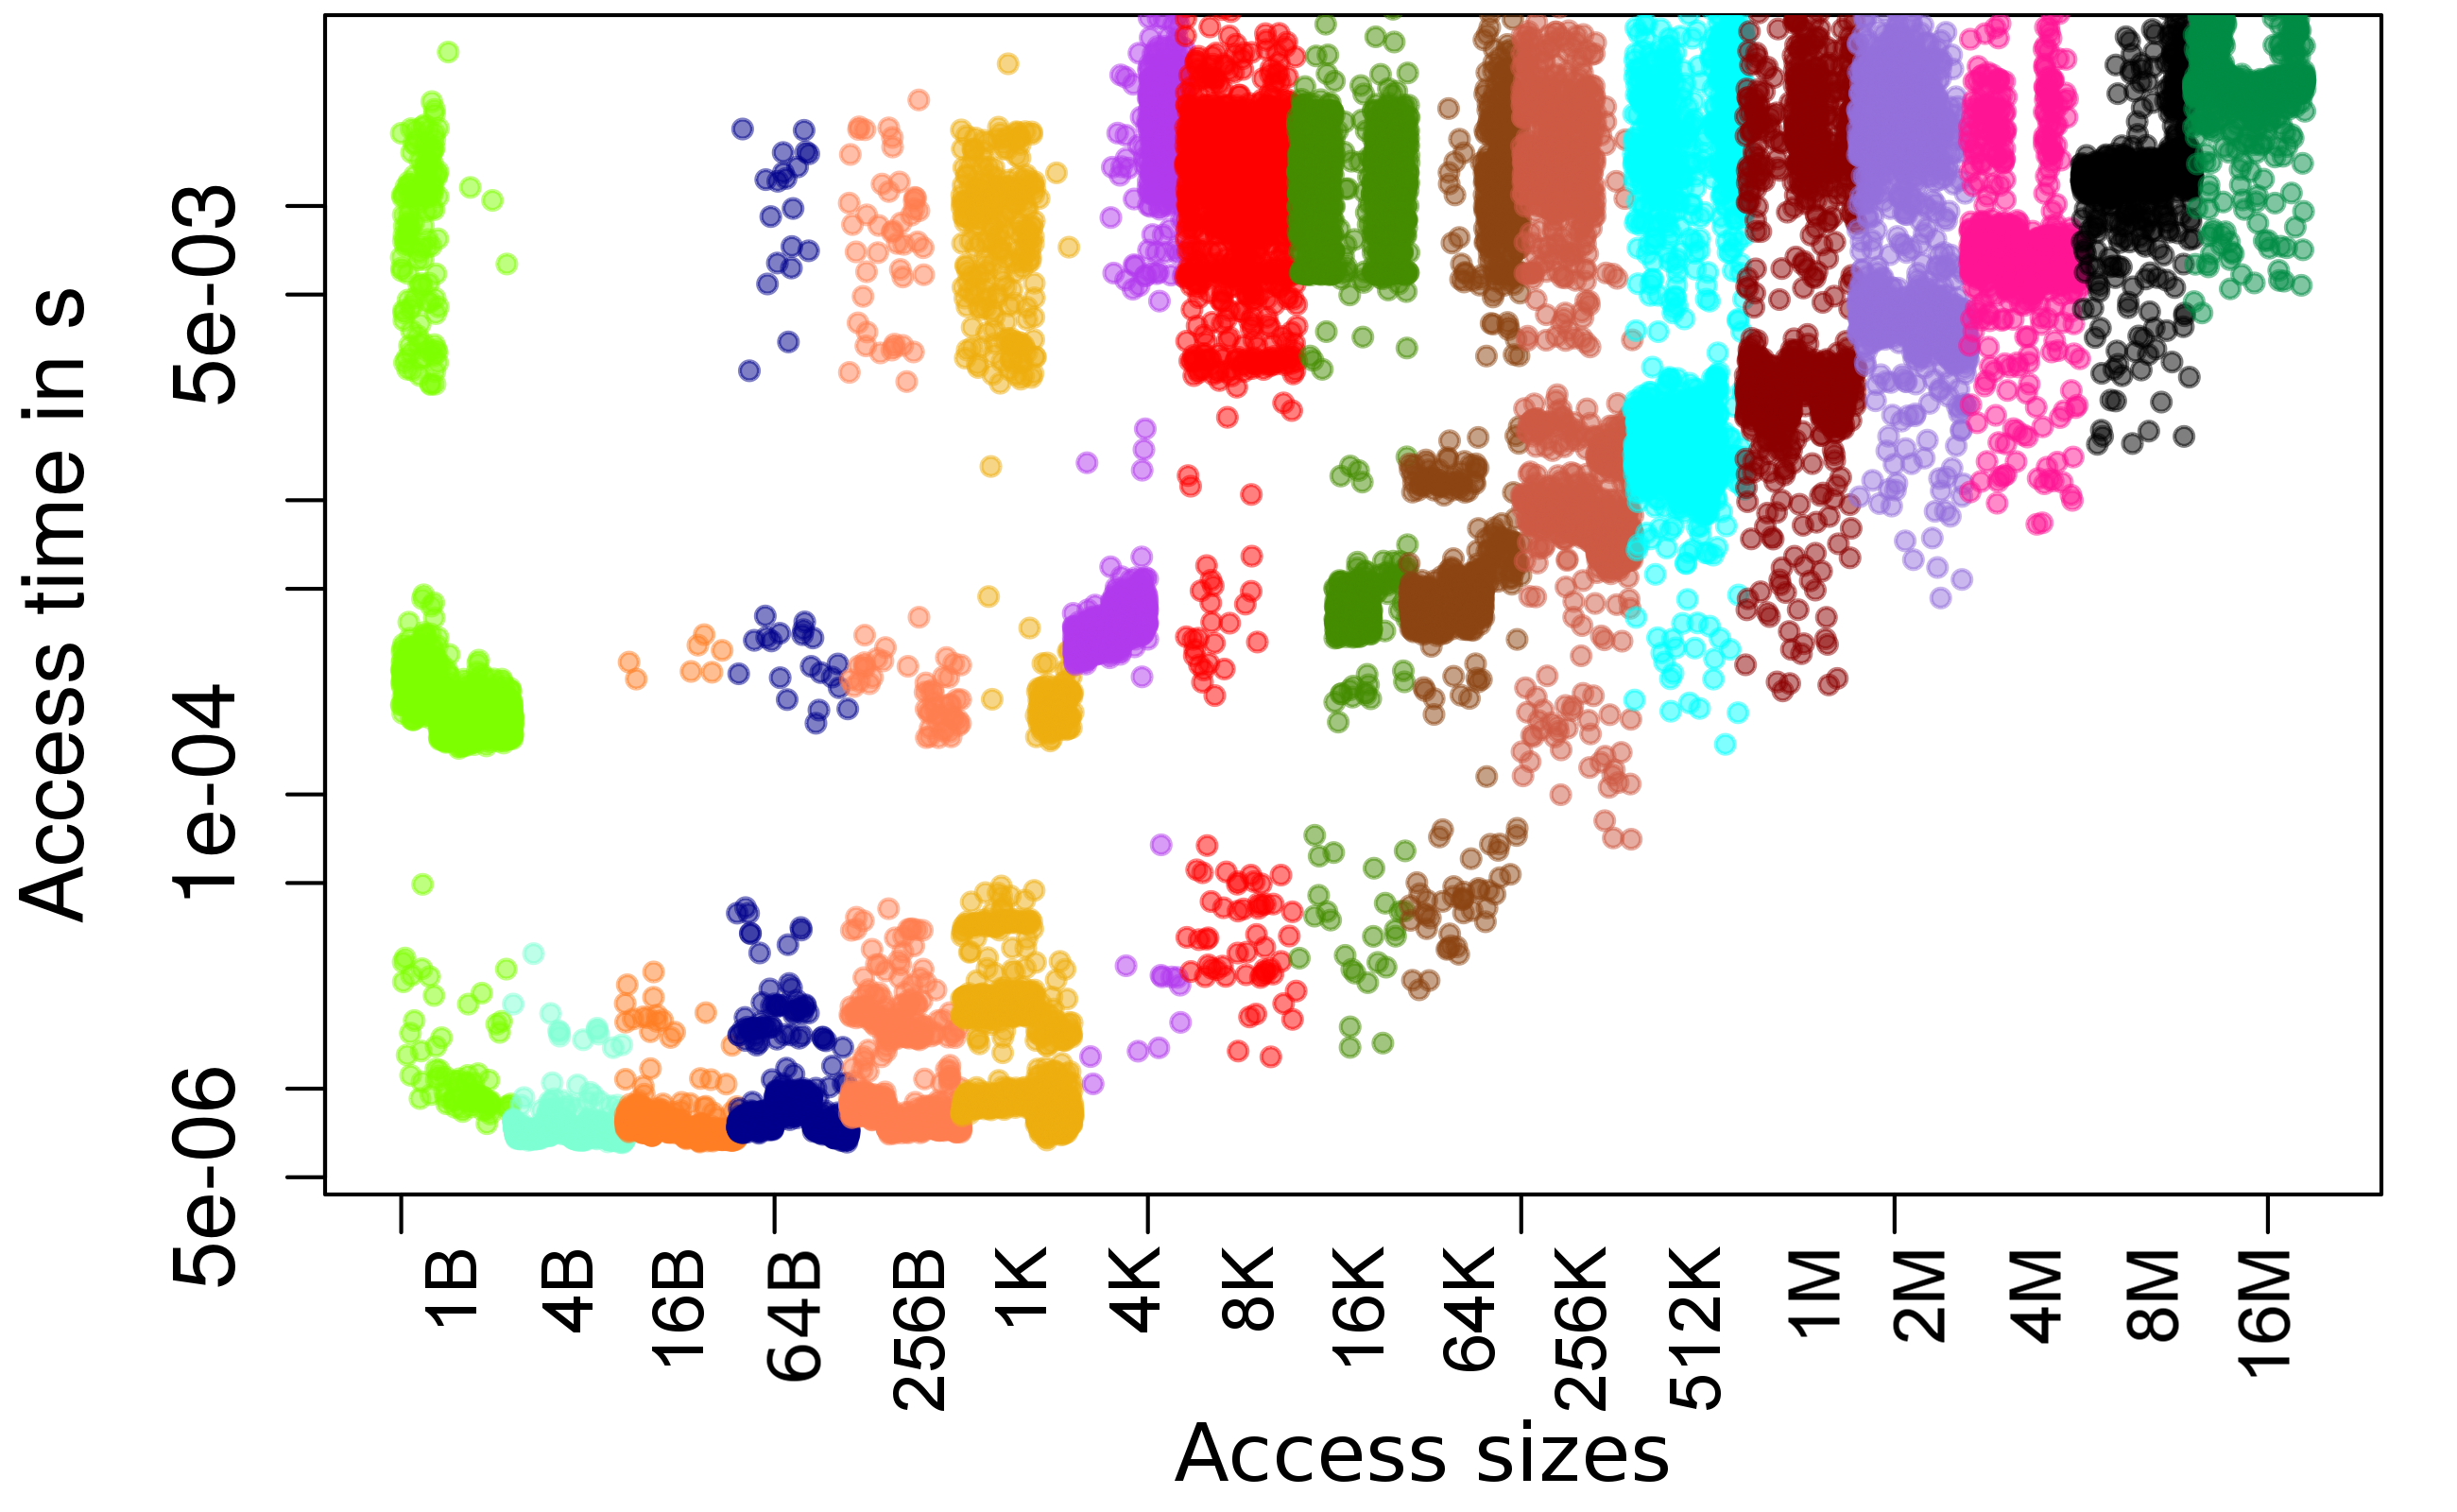
\includegraphics[width=1\linewidth]{Bilder/plot_SizeSorted_log_read_rnd.png}
	\end{figure}
\column{.45\textwidth}
	\begin{figure}
		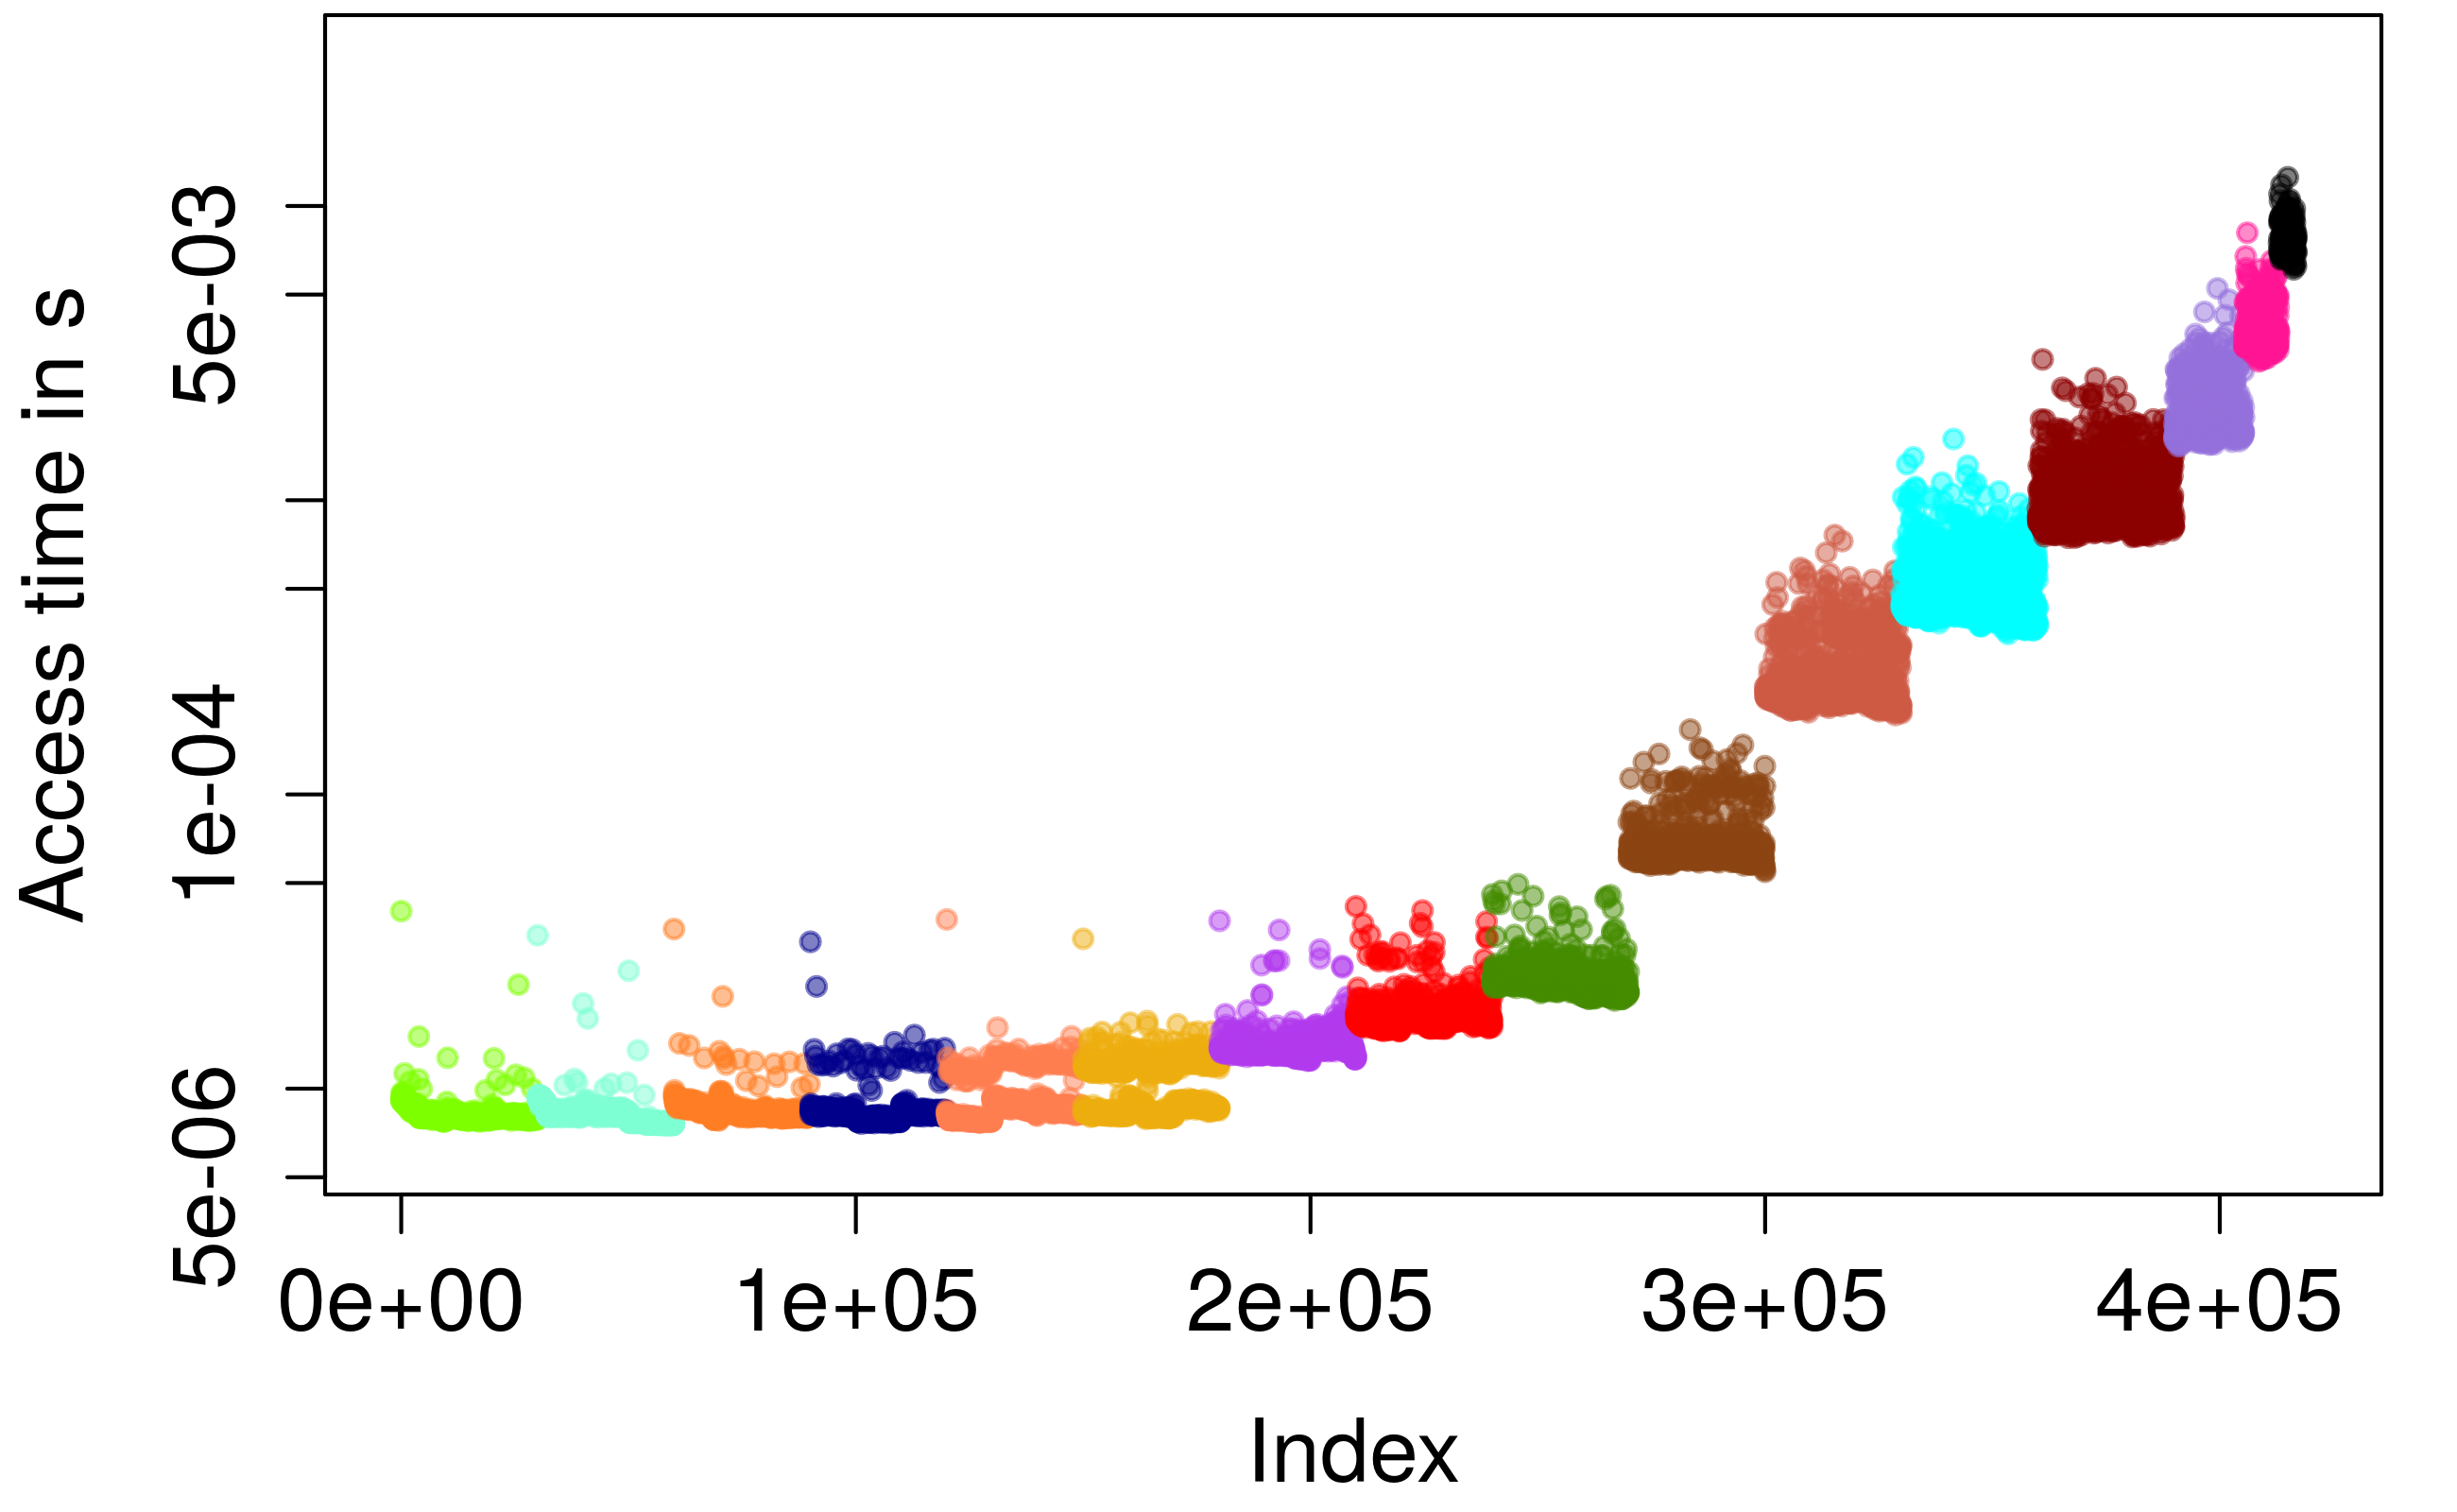
\includegraphics[width=1\linewidth]{Bilder/plot_SizeSorted_log_write_seq.png}\\
		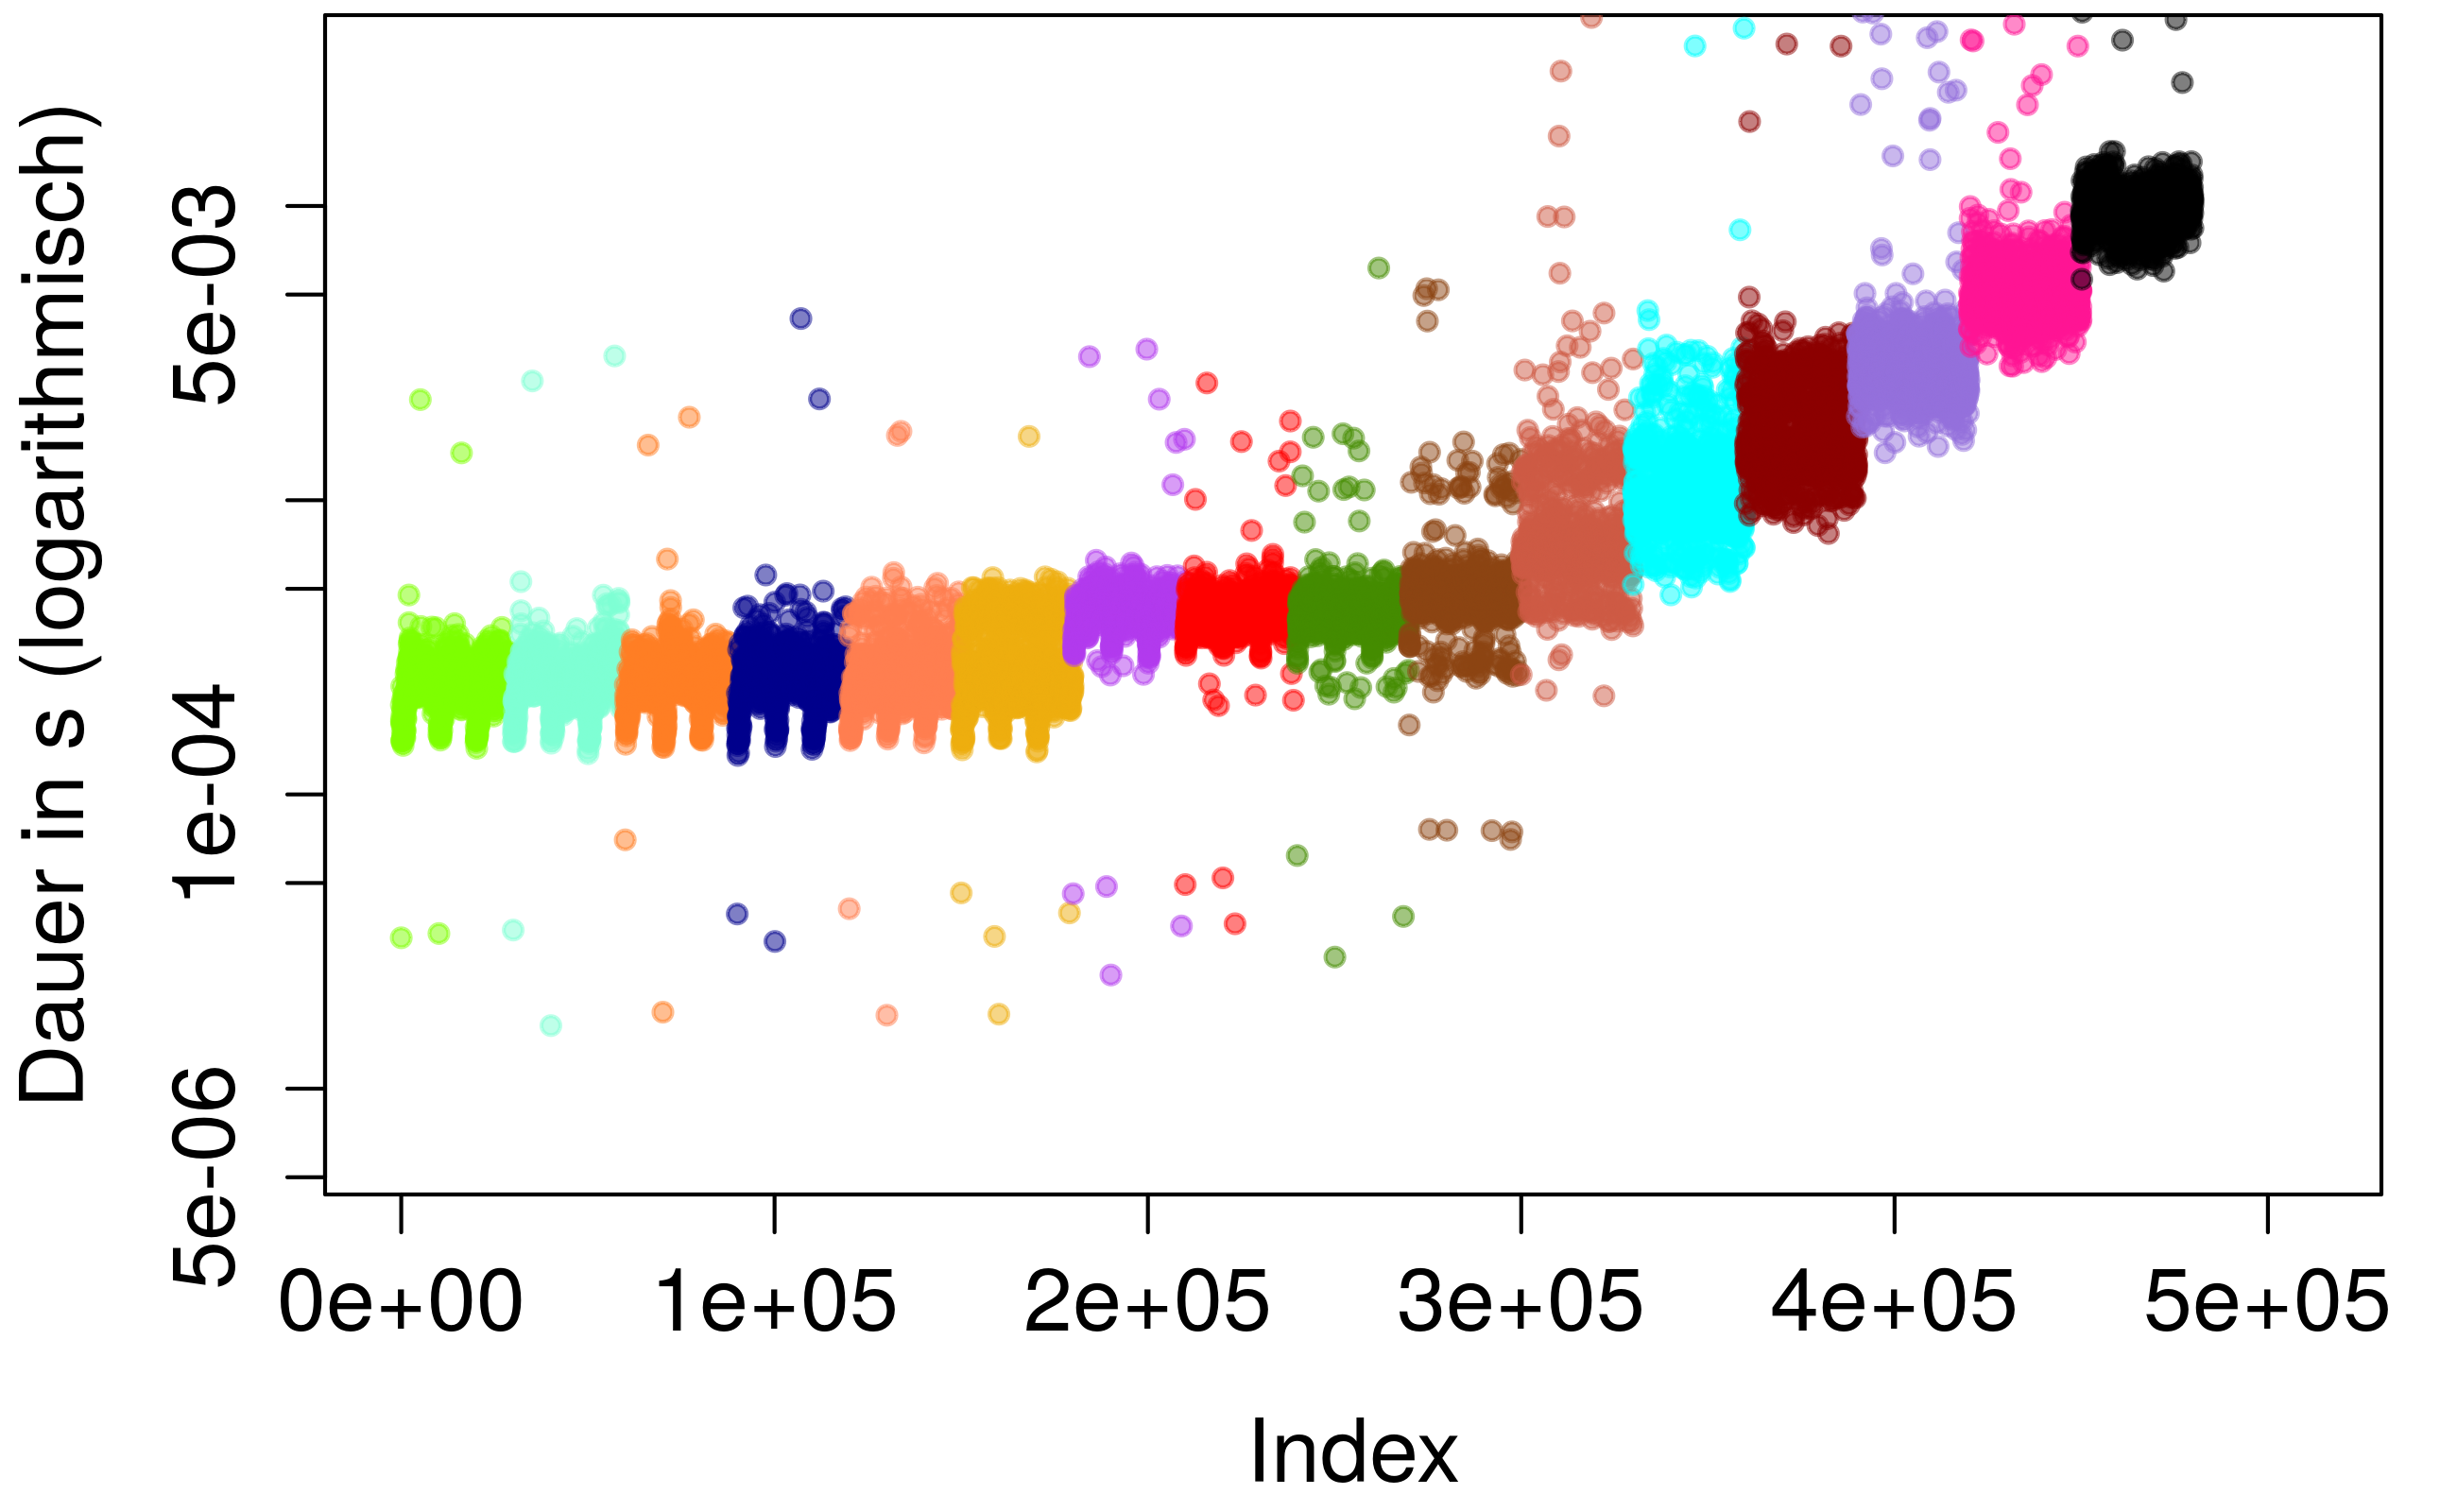
\includegraphics[width=1\linewidth]{Bilder/plot_SizeSorted_log_write_rnd.png}
	\end{figure}
	%jede Farbe eine Messgröße, im Seq Fall komplett gleiche Attribute
	%1 B, 4 B, 16 B, 64 B, 256 B, 1 KiB, 4 KiB,8 KiB, 16 KiB, 64 KiB, 256 KiB,512 KiB, 1 MiB, 2 MiB, 4 MiB,8 MiB und 16 MiB
	%Betrachtung in Zeitreihe
	%3 Messreihen direkt hintereinader
	%Starke Abhängigkeit von Zugriffsgröße erkennbar, aber muss mehr geben (RND-R)
	%deutlich zu erkennen, dass Messungen mit gleichen Attributen zu sehr unterschiedlichen ergebnissen führen können
	%Aufteilung der Messungen mit selben Attributen in über mehrere Zugriffsgrößen übergreifende Gruppen, keine gleichmäßige Verteilung wie zu erwarten wäre -> E/A-Pfad
	%Zugriffszeit stärker vom E/A-Pfad als von Zugriffsgröße abhängig
\end{columns}
\end{frame}

\section{Erste Ergebnisse}
%lineare vs nn modelle, was sind die Modelle überhaupt?

\section{E/A-Pfad zur Leistungsvorhersage}
\begin{frame}
\frametitle{E/A-Pfad zur Leistungsvorhersage}
\begin{itemize}
	\item 
\end{itemize}
\end{frame}
\subsection{Fehlerklassen}
%Verfahren zum Erstellen der FK
%Analyse der FK
\subsection{Ergebnisse von Modellen mit Fehlerklassen}

\section{Zusammenfassung und Ausblick}
%------------------------------------------------

\begin{frame}
\Huge{\centerline{Ende der Präsentation}}
\end{frame}

%----------------------------------------------------------------------------------------

\end{document} 